\documentclass[11pt, a4paper, abstract=true]{scrartcl}
\usepackage[sexy]{evan}
\usepackage{float}
\usepackage[margin=0.75in]{geometry}
\usepackage{multirow}
\def\arraystretch{1.20}

% \clearpairofpagestyles
\setkomafont{pagenumber}{\itshape}
\KOMAoptions{}
\ohead{\footnotesize \textbf{\leftmark}}
\ihead{\footnotesize \textsc{Experiment III}}
\cfoot{\pagemark}
\begin{document}
\subject{
    PH1102: Experiment III
}
\title{
    \huge Determination of \\
    Coefficient of Viscosity of Castor Oil \\ 
    Using Stokes' Law
}
\author{
    Abhisruta Maity \\
    {\normalsize 21MS006}
    \plusemail{am21ms006@iiserkol.ac.in}
}
\date{}
\publishers{
    \normalsize \emph{Indian Institute of Science Education and Research, Kolkata \\
    Mohanpur, West Bengal, 741246, India}
}
\maketitle

\tableofcontents

\newpage

\section{Briefing the Experiment}
Analogous to \emph{Elastic Moduli} and \emph{Friction} related properties of solid objects, \emph{Viscosity} is very important and one of the intrinsic properties of a liquid. It generally yields a quantitative measure of the intermolecular drag or attractive or cohesive forces of that liquid. Qualitatively, more viscous liquids shows more `stickiness' with respect to the layers of the liquid flow.

In this nice experiment, we tried to determine coefficient of viscosity of a given liquid (high-viscous castor oil) through computational linear regression with using and manipulating the database provided to us by respected instructors.

%Smaller ball such that it reaches it's terminal verlocity quicktly before reaching the bottom. Similarly, high viscous: eta high. Height of the viscometer column is small.

\section{Aim of the Experiment}
Our focusing goal of this experiment is to determine the coefficient of viscosity of a given liquid in our institutional laboratory using so-called \emph{falling ball viscometer} and incorporating Stokes' Law. Technically, in these virtual sessions, the required database of the experiment is given and we are going to analyse them remotely.

\section{Underlying Theory}
\subsection{Historical Background and Stokes' Law}
Since the era of Newton, physicists were analysing the dynamics of the bodies in different fluid media. They carefully observed that there is a concept of friction in solid–solid contact area as well as in case of solid–fluid. Sir George Stokes, 1st Baronet (1851), mathematically derived that if a spherical object moves in a medium of infinite extent (edge–effects are zero), then the drag force (\(F\)) on that object by the internal friction of the medium is directed opposite to the velocity (\(v\)) of the object, and has the magnitude
\begin{equation}
    F = 6 \pi \eta r v
\end{equation}
where \(r\) is the radius of the spherical object. Notice that, there is a constant in the expression  known as Coefficient of Viscosity (\(\eta\)). This is the quantitative measure of viscosity of the medium. As we said earlier, it describes the internal friction of a moving fluid. 

The force that opposes the relative motion between the adjacent layers of fluid (in terms of viscosity), is stated below.

\subsection{Origin of Coefficient of Viscosity}
In case of solid deformation (shear), we know that \[\text{Shear Stress} \propto \text{Shear Strain}\] hence, we can define an intrinsic property of the solid as \(\zeta\) being the \emph{Shear Modulus} satisfying \[\zeta = \frac{\text{Shear Stress}}{\text{Shear Strain}}\]

In the similar fashion, experimentalists observed that we can always find the Coefficient of Viscosity of a fluid by the following definition
\begin{equation}
    \eta \defeq \frac{\text{Shear Stress}}{\text{Sheer Strain Rate}}
    \label{eq:eq2}
\end{equation}
Note that, the denomenator is \emph{Sheer Strain Rate}, not \emph{Sheer Strain}. The fluids that follow Equation \ref{eq:eq2} are called \emph{Newtonian Fluids}\footnote{We here will analyse Newtonian liquid only. Study of non-Newtonian fluids are beyond the scope of this course.}. By some physical manipulations, the internal friction force due to viscosity of the liquid comes out to be
\begin{equation}
    \sigma = \eta \frac{\text{d}v}{\text{d}y}
\end{equation}
where \(\sigma\) is stress and \(\frac{\text{d}v}{\text{d}y}\) is velocity gradient. We have assumed the flow-bed to be planar here.\footnote{Another fomulation with circular flow-bed was found in I.E. Irodov. \emph{Problem In General Physics.} as \(\sigma = \eta r \frac{\text{d}\omega}{\text{d}r}\).}
\subsection{Dependence upon Other Thermodynamic Variables}
Viscosity depends upon temperature of the liquid. As temperature increases, the average kinetic energy of molecules of the liquid  increases, so the fluctuations, consequently,  cohesive forces decreases. Hence, viscosity decreases with increasing temperature.

\section{Working Formula}
Stokes' Law was originally derived for motion of a  spherical mass in a medium of infinite extent. But since we have finite medium in reality (liquid column here), we have to correct the formula experimentally. By virtue of various popular researches, it has been fond that, the Stokes' law takes the following form 
\begin{equation}
    F = 6 \pi \eta r v \left(1 + 2.4 \frac{r}{R}\right)\left(1 + 3.3 \frac{r}{h}\right)
\end{equation}
In our experimental setup, \(\frac{r}{R} \approx 0.1\) and \(\frac{r}{h} \approx 0.002\). We can neglect the effect of latter. Consider, the terminal velocity is achieved by the falling ball in the passage of P–Q observation, we can equate net upward and downward forces (figure below) on the ball \[6 \pi \eta r v \left(1 + 2.4 \frac{r}{R}\right) + \sigma \left(\frac{4}{3}\pi r^3\right) g = \rho \left(\frac{4}{3}\pi r^3\right) g\] A little algebraic rearrangement yields our working formula for this experiment
\begin{equation}
    \eta = \frac{2}{9} \frac{r^2(\rho - \sigma)g}{v_t (1 + 2.4\frac{r}{R})} \; \text{Poise}
    \label{eq:eq5}
\end{equation}
where \(\eta\) is the desired viscosity of given liquid, \(r\) cm is the radius of the spherical ball, \(R\) cm is the radius of the liquid column, \(\rho\) g/cm\(^3\) being the density of that ball, \(\sigma\) g/cm\(^3\) being the density of the given liquid, \(v_t\) cm/s denotes terminal velocity of the ball and \(g\) cm/s\(^2\) is the gravitational acceleration due to earth's field. A similar calculation with SI units will yield \(\eta\) in Pa s. We have \[1 \; \text{Pa s} = 10  \; \text{Poise}\]
\section{Diagram and Images of the Experiment}
\begin{figure}[H]
    \begin{minipage}{0.48\textwidth}
      \centering
      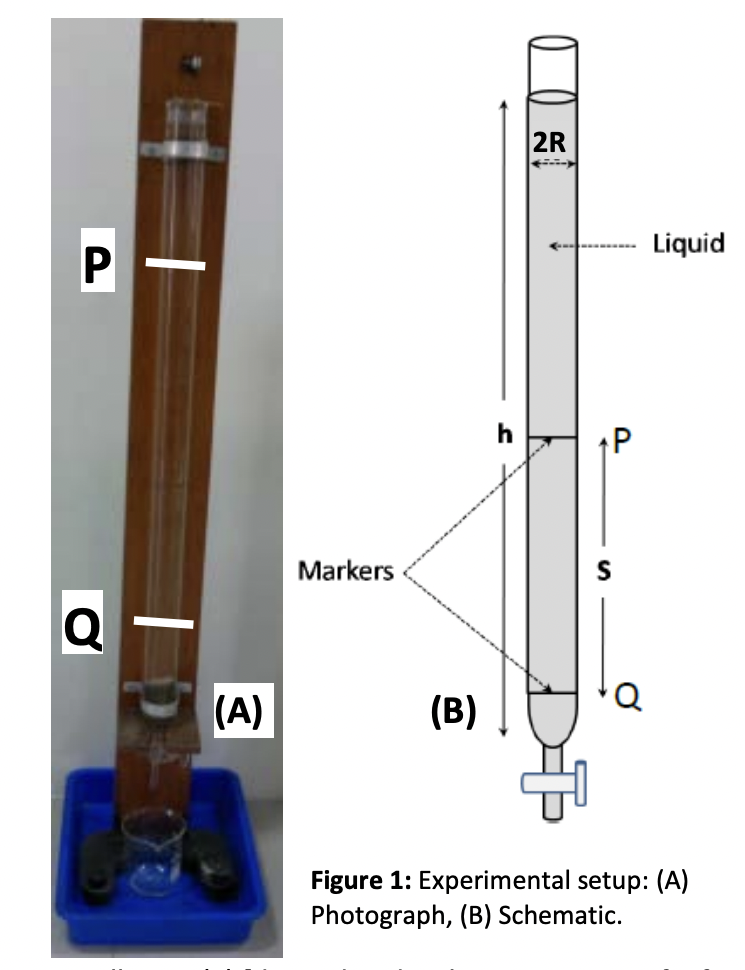
\includegraphics[width=.85\linewidth]{Apparatus.png}
    \end{minipage}\hfill
    \begin{minipage}{0.48\textwidth}
      \centering
      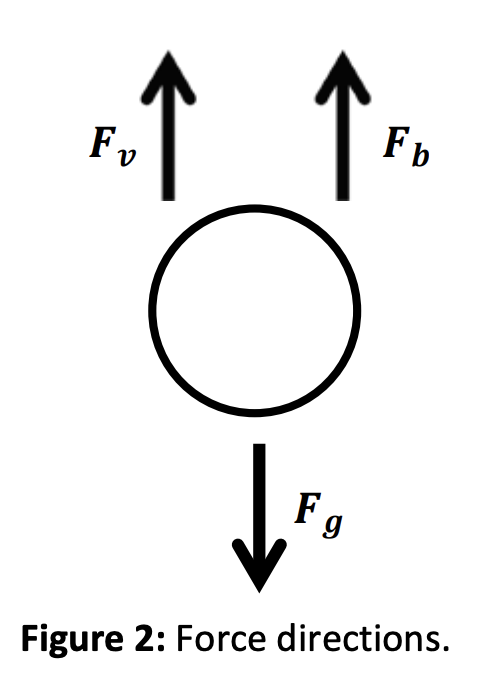
\includegraphics[width=.8\linewidth]{Force.png}
    \end{minipage}
\end{figure}
% \begin{tabular}{cc}
%     \begin{figure}
%         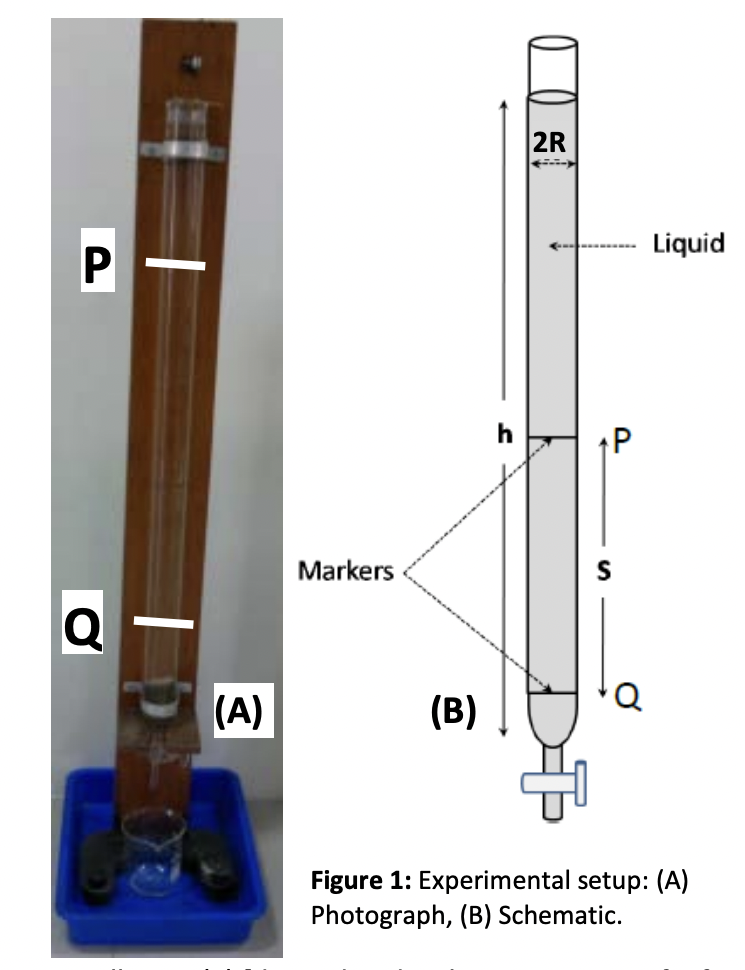
\includegraphics[scale=0.7]{Apparatus.png}
%         \label{fig:fig1}
%     \end{figure}
%     & 
%     \begin{figure}
%         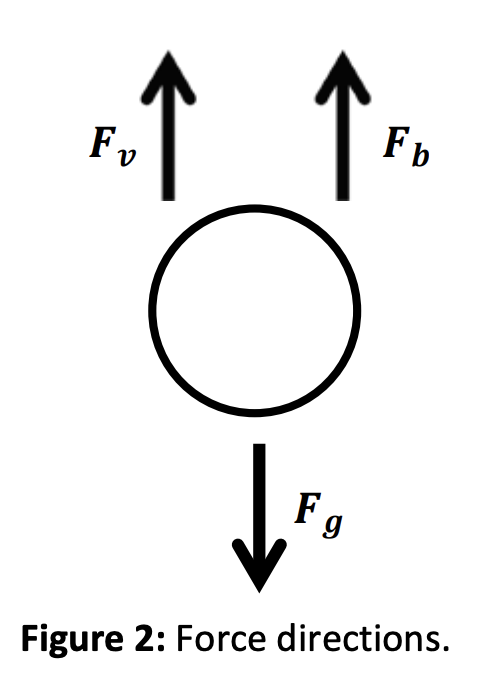
\includegraphics[scale=0.8]{Force.png}
%         \label{fig:fig2}
%     \end{figure}
% \end{tabular}
%take mean values of r and v_t

\section{Manipulating Experimental Data}
\subsection{Instrumental Data and Literature Value}
\begin{itemize}
    \item Least Count of the Screw Gauge = 0.001 cm
    \item Least Count of Digital Balance = 0.01 g
    \item Least Count of Stopwatch = 0.01 s
    \item Least Count of Meter Scale = 1 mm = 0.001 m
    \item Vernier Constant of Vernier Calliper = 0.002 cm
    \item Distance traversed by the spherical balls = 80 cm = 0.80 m
    \item Density of Castor Oil = 0.961 g/cm\(^3\) (At Room Temperature = 23 \(^{\circ}\)C)
\end{itemize}
\subsection{Parameters for Ball 1 (Small)}
\begin{table}[H]
    \centering
    \begin{tabular}{|c|ccc|c|c|}
    \hline
    No. &
      \multicolumn{1}{c|}{\begin{tabular}[c]{@{}c@{}}Linear\\ Scale\\ reading\\ (in cm)\end{tabular}} &
      \multicolumn{1}{c|}{\begin{tabular}[c]{@{}c@{}}Circular\\ Scale\\ Reading\end{tabular}} &
      \begin{tabular}[c]{@{}c@{}}Diameter\\ (in cm)\end{tabular} &
      \multicolumn{1}{c|}{\begin{tabular}[c]{@{}c@{}}Mean\\ Diameter\\ (in cm)\end{tabular}} &
      \begin{tabular}[c]{@{}c@{}}Mean\\ Radius\\ (in cm)\end{tabular} \\ \hline
    1 & 0.3 & 15 & 0.315 & \multirow{7}{*}{0.316} & \multirow{7}{*}{0.158} \\ \cline{1-1}
    2 & 0.3 & 18 & 0.318 &                        &                        \\ \cline{1-1}
    3 & 0.3 & 17 & 0.317 &                        &                        \\ \cline{1-1}
    4 & 0.3 & 15 & 0.315 &                        &                        \\ \cline{1-1}
    5 & 0.3 & 16 & 0.316 &                        &                        \\ \cline{1-1}
    6 & 0.3 & 19 & 0.319 &                        &                        \\ \cline{1-1}
    7 & 0.3 & 16 & 0.316 &                        &                        \\ \hline
    \end{tabular}
    \caption{Determination of Radius of Ball 1 (Small) using Screw Gauge}
\end{table}
\begin{table}[H]
    \def\arraystretch{1.15}
    \setlength\tabcolsep{0.5in}
    \centering
    \begin{tabular}{|c|c|}
    \hline
    \begin{tabular}[c]{@{}c@{}}Mass of \\ 10 balls \\ (in gm)\end{tabular} & \begin{tabular}[c]{@{}c@{}}Mass of\\ 1 ball\\ (in gm)\end{tabular} \\ \hline
    1.31                                                                   & 0.131                                                              \\ \hline
    \end{tabular}
    \caption{Determination of Mass of Ball 1 (Small) using Digital Balance}
\end{table}
From the above data, we found the volume of the ball = 0.0165 cm\(^3\). 

\setlength{\parindent}{0in} Subsequently, we found the density = 7.94 g/cm\(^3\).
% Please add the following required packages to your document preamble:
% \usepackage{multirow}
\begin{table}[H]
    \setlength\tabcolsep{0.33in}
    \centering
    \begin{tabular}{|c|c|c|}
    \hline
    No. & \begin{tabular}[c]{@{}c@{}}Time for\\ Ball 1\\ (in s)\end{tabular} & \begin{tabular}[c]{@{}c@{}}Avg. Time\\ Duration\\ (in s)\end{tabular} \\ \hline
    1 & 15.72 & \multirow{7}{*}{15.84} \\ \cline{1-2}
    2 & 15.93 &                        \\ \cline{1-2}
    3 & 15.88 &                        \\ \cline{1-2}
    4 & 15.85 &                        \\ \cline{1-2}
    5 & 15.75 &                        \\ \cline{1-2}
    6 & 16.03 &                        \\ \cline{1-2}
    7 & 15.78 &                        \\ \hline
    \end{tabular}
    \caption{Determination of Time Elasped by Ball 1 (Small) using Stopwatch}
\end{table}
Hence, we found the terminal velocity of the ball = 5.05 cm/s = 0.0505 m/s.

\subsection{Parameters for Ball 2 (Medium)}
\begin{table}[H]
    \centering
    \begin{tabular}{|c|ccc|c|c|}
    \hline
    No. &
      \multicolumn{1}{c|}{\begin{tabular}[c]{@{}c@{}}Linear\\ Scale\\ reading\\ (in cm)\end{tabular}} &
      \multicolumn{1}{c|}{\begin{tabular}[c]{@{}c@{}}Circular\\ Scale\\ Reading\end{tabular}} &
      \begin{tabular}[c]{@{}c@{}}Diameter\\ (in cm)\end{tabular} &
      \begin{tabular}[c]{@{}c@{}}Mean\\ Diameter\\ (in cm)\end{tabular} &
      \begin{tabular}[c]{@{}c@{}}Mean\\ Radius\\ (in cm)\end{tabular} \\ \hline
    1 & 0.3 & 48 & 0.348 & \multirow{7}{*}{0.348} & \multirow{7}{*}{0.174} \\ \cline{1-1}
    2 & 0.3 & 46 & 0.346 &                        &                        \\ \cline{1-1}
    3 & 0.3 & 49 & 0.349 &                        &                        \\ \cline{1-1}
    4 & 0.3 & 46 & 0.346 &                        &                        \\ \cline{1-1}
    5 & 0.3 & 48 & 0.348 &                        &                        \\ \cline{1-1}
    6 & 0.3 & 49 & 0.349 &                        &                        \\ \cline{1-1}
    7 & 0.3 & 47 & 0.347 &                        &                        \\ \hline
    \end{tabular}
    \caption{Determination of Radius of Ball 2 (Medium) using Screw Gauge}
\end{table}
\begin{table}[H]
    \def\arraystretch{1.15}
    \setlength\tabcolsep{0.5in}
    \centering
    \begin{tabular}{|c|c|}
    \hline
    \begin{tabular}[c]{@{}c@{}}Mass of \\ 10 balls \\ (in gm)\end{tabular} & \begin{tabular}[c]{@{}c@{}}Mass of\\ 1 ball\\ (in gm)\end{tabular} \\ \hline
    2.05                                                                   & 0.205                                                              \\ \hline
    \end{tabular}
    \caption{Determination of Mass of Ball 2 (Medium) using Digital Balance}
\end{table}
From the above data, we found the volume of the ball = 0.0221 cm\(^3\). 

\setlength{\parindent}{0in} Subsequently, we found the density = 9.28 g/cm\(^3\).
% Please add the following required packages to your document preamble:
% \usepackage{multirow}
\begin{table}[H]
    \setlength\tabcolsep{0.33in}
    \centering
    \begin{tabular}{|c|c|c|}
    \hline
    No. & \begin{tabular}[c]{@{}c@{}}Time for\\ Ball 1\\ (in s)\end{tabular} & \begin{tabular}[c]{@{}c@{}}Avg. Time\\ Duration\\ (in s)\end{tabular} \\ \hline
    1 & 10.66 & \multirow{7}{*}{10.64} \\ \cline{1-2}
    2 & 10.65 &                        \\ \cline{1-2}
    3 & 10.69 &                        \\ \cline{1-2}
    4 & 10.57 &                        \\ \cline{1-2}
    5 & 10.66 &                        \\ \cline{1-2}
    6 & 10.63 &                        \\ \cline{1-2}
    7 & 10.59 &                        \\ \hline
    \end{tabular}
    \caption{Determination of Time Elasped by Ball 2 (Medium) using Stopwatch}
\end{table}

Hence, we found the terminal velocity of the ball = 7.52 cm/s = 0.0752 m/s.

\subsection{Parameters for Ball 3 (Large)}
\begin{table}[H]
    \centering
    \begin{tabular}{|c|ccc|c|c|}
    \hline
    No. &
      \multicolumn{1}{c|}{\begin{tabular}[c]{@{}c@{}}Linear\\ Scale\\ reading\\ (in cm)\end{tabular}} &
      \multicolumn{1}{c|}{\begin{tabular}[c]{@{}c@{}}Circular\\ Scale\\ Reading\end{tabular}} &
      \begin{tabular}[c]{@{}c@{}}Diameter\\ (in cm)\end{tabular} &
      \begin{tabular}[c]{@{}c@{}}Mean\\ Diameter\\ (in cm)\end{tabular} &
      \begin{tabular}[c]{@{}c@{}}Mean\\ Radius\\ (in cm)\end{tabular} \\ \hline
    1 & 0.4 & 24 & 0.424 & \multirow{7}{*}{0.426} & \multirow{7}{*}{0.213} \\ \cline{1-1}
    2 & 0.4 & 26 & 0.426 &                        &                        \\ \cline{1-1}
    3 & 0.4 & 28 & 0.428 &                        &                        \\ \cline{1-1}
    4 & 0.4 & 24 & 0.424 &                        &                        \\ \cline{1-1}
    5 & 0.4 & 28 & 0.428 &                        &                        \\ \cline{1-1}
    6 & 0.4 & 26 & 0.426 &                        &                        \\ \cline{1-1}
    7 & 0.4 & 24 & 0.424 &                        &                        \\ \hline
    \end{tabular}
    \caption{Determination of Radius of Ball 3 (Large) using Screw Gauge}
\end{table}
\begin{table}[H]
    \def\arraystretch{1.15}
    \setlength\tabcolsep{0.5in}
    \centering
    \begin{tabular}{|c|c|}
    \hline
    \begin{tabular}[c]{@{}c@{}}Mass of \\ 10 balls \\ (in gm)\end{tabular} & \begin{tabular}[c]{@{}c@{}}Mass of\\ 1 ball\\ (in gm)\end{tabular} \\ \hline
    4.47                                                                   & 0.447                                                              \\ \hline
    \end{tabular}
    \caption{Determination of Mass of  Ball 3 (Large) using Digital Balance}
\end{table}
From the above data, we found the volume of the ball = 0.0405 cm\(^3\). 

\setlength{\parindent}{0in} Subsequently, we found the density = 11.04 g/cm\(^3\).

% Please add the following required packages to your document preamble:
% \usepackage{multirow}
\begin{table}[H]
    \setlength\tabcolsep{0.33in}
    \centering
    \begin{tabular}{|c|c|c|}
    \hline
    No. & \begin{tabular}[c]{@{}c@{}}Time for\\ Ball 1\\ (in s)\end{tabular} & \begin{tabular}[c]{@{}c@{}}Avg. Time\\ Duration\\ (in s)\end{tabular} \\ \hline
    1 & 7.68 & \multirow{7}{*}{7.78} \\ \cline{1-2}
    2 & 7.81 &                       \\ \cline{1-2}
    3 & 7.72 &                       \\ \cline{1-2}
    4 & 7.81 &                       \\ \cline{1-2}
    5 & 7.82 &                       \\ \cline{1-2}
    6 & 7.69 &                       \\ \cline{1-2}
    7 & 7.90 &                       \\ \hline
    \end{tabular}
    \caption{Determination of Time Elasped by Ball 3 (Large) using Stopwatch}
\end{table}
Hence, we found the terminal velocity of the ball = 10.28 cm/s = 0.1028 m/s.

\subsection{Parameter of Glass Cylinder}

\begin{table}[H]
    \setlength\tabcolsep{0.20in}
    \centering
    \begin{tabular}{|c|c|c|c|}
    \hline
    No. & \begin{tabular}[c]{@{}c@{}}Main Scale\\ Reading\\ (in cm)\end{tabular} & \begin{tabular}[c]{@{}c@{}}Vernier \\ Scale\\ Reading\end{tabular} & \begin{tabular}[c]{@{}c@{}}Diameter\\ (in cm)\end{tabular} \\ \hline 
    1 & 4.6 & 5 & 4.610 \\ \hline
    2 & 4.6 & 5 & 4.610 \\ \hline
    3 & 4.6 & 4 & 4.608 \\ \hline
    \end{tabular}
    \caption{Determination of Radius of Glass Cylinder using Vernier Caliper}
\end{table}
From the above data, we found the mean diameter of the glass cylinder = 4.610 cm and consequently, the mean radius = 2.305 cm.

\newpage

\section{Plots}
As the theory we discussed above, we expect a linear relation between \(v_t\) vs. \(r^2\), where \(v_t\) is the terminal velocities of the respective balls and \(r\) is the radius of the radius of the respective balls.

\begin{table}[H]
    \setlength\tabcolsep{0.33in}
    \centering
    \begin{tabular}{|c|c|c|}
    \hline
    No. &
      \begin{tabular}[c]{@{}c@{}}Terminal\\ Velocity \(v_t\)\\ (in cm/s)\end{tabular} &
      \begin{tabular}[c]{@{}c@{}}Square of \\ Radius \(r^2\)\\ (in cm\(^2\))\end{tabular} \\ \hline
    1 & 5.05 & 0.0250 \\ \hline
    2 & 7.52 & 0.0303 \\ \hline
    3 & 10.64 & 0.0454 \\ \hline
    \end{tabular}
    \caption{Derived \(v_t\) vs. \(r^2\) Dataset}
\end{table}

\begin{figure}[H]
    \centering
    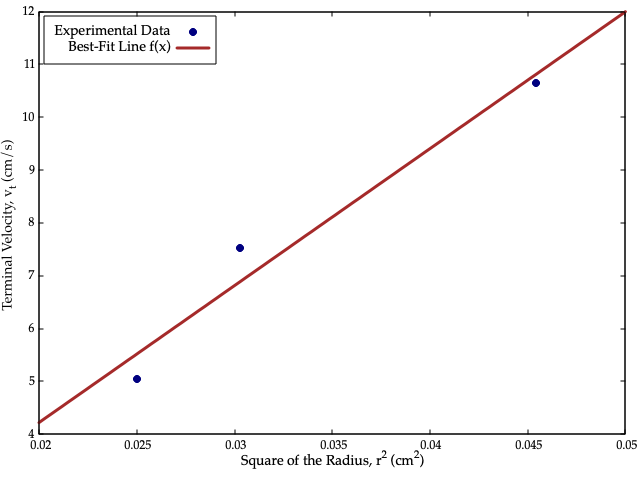
\includegraphics[scale=0.60]{plot.png}
\end{figure}

\section{Deducing Coefficient of Viscosity}
We use Equation \ref{eq:eq5} to derive viscosity of given liquid for each of three cases of the three balls. Suppose, they are \(\eta_1, \eta_2\) and \(\eta_3\) respectively. Observe that,
\begin{align*}
    \eta_1 = \frac{2}{9} \times \frac{(0.158)^2 \times(7.94 - 0.961) \times 980}{5.05 \times (1 + 2.4 \times \frac{0.158}{2.305})} \; \text{Poise} = 6.45 \; \text{Poise} = 0.645 \; \text{Pa s}
\end{align*}
\begin{align*}
    \eta_2 = \frac{2}{9} \times \frac{(0.174)^2 \times(9.28 - 0.961) \times 980}{7.52 \times (1 + 2.4 \times \frac{0.174}{2.305})} \; \text{Poise} = 6.18 \; \text{Poise} = 0.618 \; \text{Pa s}
\end{align*}
\begin{align*}
    \eta_3 = \frac{2}{9} \times \frac{(0.213)^2 \times(11.04 - 0.961) \times 980}{10.28 \times (1 + 2.4 \times \frac{0.213}{2.305})} \; \text{Poise} = 7.93 \; \text{Poise} = 0.793 \; \text{Pa s}
\end{align*}

Using the above viscosity values, we take average of them to determine the final experimental value \[\boxed{\eta = \frac{\sum_{i=1}^3 \eta_i}{3} = 0.685 \; \text{Pa s}}\]
 
\section{Estimation of Error}
\subsection{Literature Value Error}
We are given the literature value of coefficient of viscosity of Castor Oil = 0.650 \text{Pa s}. Hence, \[\%\text{Error} = \frac{0.685 - 0.650}{0.650} \times 100 = \boxed{5.38}\]
\subsection{Instrumental Error}
Due to least count of the instruments and limitations in observation strategy, there is an instrumental error whose expression can be found using logarithmic derivatives. Finally, the expression comes out to be
\begin{equation*}
    \frac{\delta\eta}{\eta} = \left|\frac{2}{r} - \frac{2.4}{R+2.4r} - \frac{9m}{4\pi r^4(\rho - \sigma)}\right|\delta r + \left|\frac{1}{x}\right|\delta x + \left|\frac{1}{t}\right|\delta t + \left|\frac{2.4r}{R(R+2.4r)}\right|\delta R + \left|\frac{3}{4\pi r^3(\rho - \sigma)}\right|\delta m
\end{equation*}
where, \(\rho = \frac{m}{\frac{4}{3}\pi r^3}\) and \(v_t = \frac{x}{t}\) with \(x\) being the column length under observation and \(t\) being time time taken by the ball to pass that column.
\begin{remark}
    We are taking \(\delta t = 0.2\) s as conservative error bound due to neurological reaction time of human observer.
\end{remark}
From this \emph{pathological} expression, error in \(\eta_i\)s comes out to be 
\begin{align*}
    \%\text{Error in } \eta_1 &= 11.78 \\ \%\text{Error in } \eta_2 &= 9.28 \\ \%\text{Error in } \eta_3 &= 7.13
\end{align*}
With the mean value of the error as \[\langle\%\text{Error in } \eta_i\rangle = \boxed{9.40}\]
%take deltat = 0.2 s, deltax = 1 mm
%sigma is given, rho have deltarho = 0  

\section{Discussion on Probable Sources of Errors}
\begin{enumerate}
    \item Since handling of the stopwatch is executed by human nervous system [Observation by Eyes \(\rightarrow\) Visual Cortex \(\rightarrow\) Motor Neurons \(\rightarrow\) Action of Start/Stop], there is an error in reading of time arises due to reaction time. If the experimentalist is very careful, then the maximum bound of this reaction time is approximately 0.2 s. This may cause inaccuracy. This can be fixed using some other (maybe computer programme-based) handling system of the stopwatch.
    \item Errors also may arise due to low resolution of instruments which are used in this experiment. It can be fixed using highly precise instruments.
    \item We can observe there is huge error in density of steel balls of three different sizes, which may be caused by rusting, oxidation, distorted geometry (non-spherical) etc. This may be fixed using round, carefully-reserved and pure-steel balls.
\end{enumerate}
\section{Conclusion and Acknowledgement}
\textsc{Thanks} to the instructors and teaching assistants for rewarding us this simple but beautiful experiment, where we experimentally calculated the value of coefficient of viscosity of a high-viscous liquid, namely \emph{Castor Oil} with significantly low amount of overall error.

\end{document}

% 11.78
% 9.28
% 7.13